\documentclass[a4paper,11pt]{article}
%
%--------------------   start of the 'preamble'
%
\usepackage{graphicx,amssymb,amstext,amsmath}
\usepackage{url}
%
%%    homebrew commands -- to save typing
\newcommand\etc{\textsl{etc}}
\newcommand\eg{\textsl{eg.}\ }
\newcommand\etal{\textsl{et al.}}
\newcommand\Quote[1]{\lq\textsl{#1}\rq}
\newcommand\fr[2]{{\textstyle\frac{#1}{#2}}}
%
%---------------------   end of the 'preamble'
%
\begin{document}
%-----------------------------------------------------------
\title{
  \textbf{\large Similarity Search Project Report}\\
  Comparison of Matching Algorithms
}

\author{Lukas Siemon and Laura Bledaite}
\maketitle

\begin{abstract}
Required or not?
\end{abstract}

\section{Introduction}

When integrating data from different sources, the exact matching of data items representing the same real world object fails often because of the missing global keys and/or different data representations. In many cases these items have attributes that can be used to automatically generate similarity values for the cross product. The next question then is how to match the items using these similarity values. In this project we discuss different techniques for this matching using a similarity matrix. Each data item from one set can be matched at most to one data item from the other set and matching is a symmetric property. This matching problem is of interest in a number of areas.

% do we want to add examples here (?)
We implement and compare four matching algorithms: Reverse Nearest Neighbor, Global Greedy, Stable Marriage, and the Hungarian Algorithm. 
The differences of the matching algorithms are then discussed by performing runtime and quality tests using our implementation. For the runtime tests we generate random matrices and for the quality test we use real-world data.

% The main objective is to match similar strings based on their distances. Possible applications include object identification in different databases, error correction in the text, finding matches for the queries with a spelling mistake \etc.
 
% The comparison of algorithms include runtime and quality tests. In our runtime tests we use randomly generated distance data of different sizes, namely: 10, 100, 1000. In the quality tests, we use Bolzano Address Tree distance data and compute recall and precision for all the algorithms.

\section{Algorithms}

\subsection{Reverse Nearest Neighbor}

The Reverse Nearest Neighbor algorithm is the only algorithm that does not match as many objects as possible.
An object $A$ is only matched to object $B$ if the object $A$ is unique, most similar object to $B$ and vice versa. In other words the matrix entry for $AB$ is the unique, smallest entry in this row and column.

The formalized details of the algorithm can be found in \cite[p. 29]{rnn}.
  
\subsection{Global Greedy}

% string -> object
The Global Greedy algorithm first sorts all possible matches ascending by similarity. It then iterates through the pairs and matches a pair if possible. A pair can be matched if there exists no other match using the same row or column.

This algorithm matches as many strings as possible, i.e min(\#rows, \#columns). Therefore, it would match even very different strings, if there are no better matches left. The algorithm yields a stable matching, which is proven in \cite{augsten}.

%The Global Greedy algorithm initially sorts the string pairs by their distance and stores them in an array. In the beginning the closest string pair is matched. The respective row and column are marked in the distance matrix to avoid a situation that a string is matched twice. The remaining string pairs in an array are matched in ascending order of their distances if both strings in the pair are still available. This algorithm matches as many strings as possible, i.e $min(\#rows, \#columns)$. Therefore, it would match even very different strings, if there are no better matches left. The algorithm yields a stable matching, which is proven in \cite{augsten}.

The Global Greedy matching algorithm requires $O(N^2)$ space (the size of the distance matrix) and runs in $O(N^2 log(N))$ time (sorting the distances).

\subsection{Stable Marriage}

% string -> object
The Stable Marriage algorithm was first presented in \cite{gale}. One of the application examples was the assignments of students to the colleges given a quota for each college and the preferential rankings of both sides. The special case of a problem, when there is the same number of studends and colleges and all the quotas are unity was explained as a situation when the equal number of men and women seek for a partner based on their ranking lists.

The latter case is readily applicable for the string matching problem. The difference is that for matching strings the input is a distance matrices. Therefore, to use the algorithm the row-wise and column-wise rankings of the distances have to be calculated (the smaller the distance, the better the ranking).

Further, the algorithm is identical to the original stable marriage. Suppose, that there are less columns than rows in the distence matrix. If not, then transpose the distance matrix and follow the same procedure. Also, imagine that rows represent boys, and columns represent girls. To start, each boy finds its best ranked girl. Each girl who receives more than one proposal rejects all but her favorite from among those who have proposed to her. However, she does not accept him yet, but keeps him on a string to allow for the possibility that someone better may come along later.

In the second stage those boys who were rejected now propose to their second choices. Each girl receiving proposals chooses her favorite from the group consisting of the new proposers and the boy on her string, if any. She rejects all the rest and again keeps the favorite in suspense.

We proceed in the same manner. Those who are rejected at the current stage propose to their next choices, and the girls again reject all but the best proposal they have had so far.

%\textit{//Can be proven that it terminates?}
One question regarding the Stable Marriage algorithm is whether it can be proven that the algorithm terminates. Once a girl receives a proposal, she remains engaged, but may chenge her mind for a better proposal. Therefore, from the girls' point of view this algorithm is greedy. In every iteration a boy will eliminate one of his choices. As a result, if it continues for long enough, at some point there will be no girls left to propose. Therefore, at the end $min(\#girls, \#boys)$, i.e. the maximum number of pairs, will be matched and the algorithm terminates.


\subsection{Hungarian Algorithm}

The algorithm was first published in \cite{ha_firstpub}.

The basic idea is to assign the objects in such a way that the overall cost of all assignments is minimal, e.g. the sum of all used similarity values is minimal. This means that an object is not assigned to it's best match if the overall cost of all assignments can be reduced that way. The algorithm further matches as many pairs as possible.

% I use capital N, because later I say that N is max(n,m)
Our implementation, which runs in $O(N^4)$, is loosely based on the original algorithm and  \url{http://csclab.murraystate.edu/bob.pilgrim/445/munkres.html}. It is known that the algorithm can be implemented to run in $O(N^3)$, but for us the (well studied) original algorithm was sufficient. Further it is noticeable that we did not find a Java implementation that runs in $O(N^3)$. An existing Java implementations\footnote{\url{http://konstantinosnedas.com/dev/soft/munkres.htm}} that claimed to achieve $O(n^{3})$, showed that it was in fact running in $O(n^{4})$.

The details of the algorithm are not described here. However the basic idea is to decrease the size of the entries in the cost matrix in an intelligent way. When the algorithm terminates, there is a marked zeros for every match. 

\section{Experiments}

The comparison of the algorithms includes runtime and quality tests. In our runtime tests we use randomly generated distance matrices of increasing size. In the quality tests, we use Bolzano Address Tree distance data and compute recall and precision for all four algorithms.

\subsection{Runtime Tests}

In all graphs in this section the y-axis ($n$) represents the size of a $n \times n$ test-matrix. The matrix is generated using random double values in $[0,1]$ as entries. We use a logarithmic scale for easier interpretation.

\subsubsection{Reverse Nearest Neighbor}

\begin{figure}[ht!]
\centering 
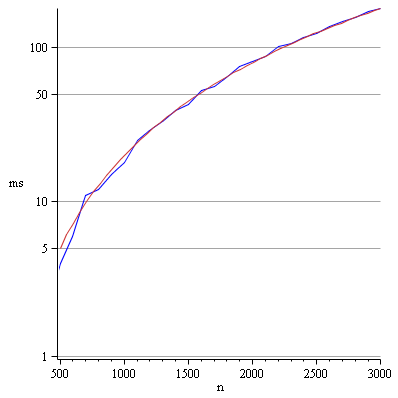
\includegraphics[width=80mm]{RNN_runtime.png}
\caption{The running time of the Reverse Nearest Neighbor algorithm fitted to $x^2$.}
\label{rnn} 
\end{figure}

The blue graph in Figure~\ref{rnn} represents the runtime of our RNN implementation. The orange curve is a fitted $x^2$ function. As expected, the complexity of the algorithm is $O(N^{2})$.

\subsubsection{Global Greedy}

\begin{figure}[ht!]
\centering 
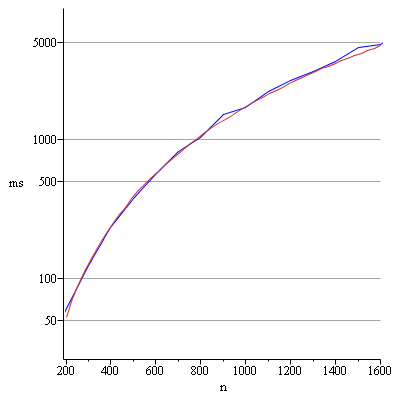
\includegraphics[width=80mm]{GG_runtime.png}
\caption{The running time of the Global Greedy algotithm fitted to $x^2 \cdot log(x)$.}
\label{gg} 
\end{figure}

The blue graph in Figure~\ref{gg} represents the runtime of our GG implementation. The orange curve is a fitted $x^2 \cdot log(x)$ function. As expected, the complexity of the algorithm is $O(N^{2} \cdot log(N))$, which comes from sorting the distances.

\subsubsection{Stable Marriage}

\begin{figure}[ht!]
\centering 
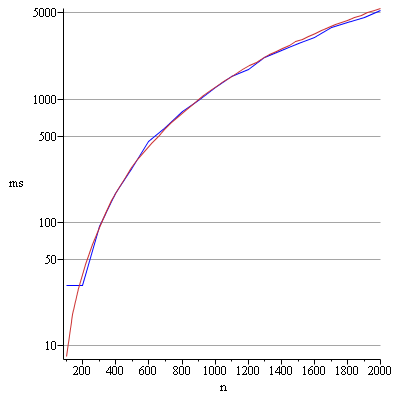
\includegraphics[width=80mm]{SM_runtime.png}
\caption{The running time of the Stable Marriage algotithm fitted to $x^2 \cdot log(x)$.}
\label{sm} 
\end{figure}

The blue graph in Figure~\ref{sm} represents the runtime of our Stable Marriage algotithm implementation. The orange curve is a fitted $x^2 \cdot log(x)$ function. As expected, the complexity of the algorithm is $O(N^{2} \cdot log(N))$, which comes from preparing the input matrix for the algorithm. We have to sort the rows and columns.

  If the distance matrix is $n$x$m$, then to sort one row takes $m \cdot log(m)$ time. Similarly, to sort one column, it takes $n \cdot log(n)$ time. Therefore, the sorting takes $m \cdot n \cdot log(n) + n \cdot m \cdot log(m)$. Thus, if we denote the maximum of $n$ and $m$ by $N$, the time required for sorting is $O(N^{2} \cdot log(N))$. 

The complexity of the original algorithm was proven to be $N^{2}$. Hence we notice that applying the algorithm to our specific problem increases the complexity. The increase is not very significant though.

\subsubsection{Hungarian Algorithm}

\begin{figure}[ht!]
\centering 
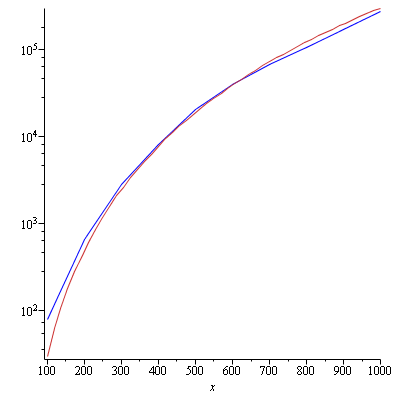
\includegraphics[width=80mm]{HA_runtime.png}
\caption{The running time of the Hungarian algotithm fitted to $x^4$.}
\label{hung} 
\end{figure}

The blue graph in Figure~\ref{hung} represents the runtime of our HA implementation. The orange curve is a fitted $x^4$ function. As expected, the complexity of the algorithm is $O(n^{4})$. Note that it is possible to implement the Hungarian Algorithm in $O(n^{3})$.

The higher complexity compared to the other matching algorithms is because the Hungarian algorithm aims to assign the objects in such a way that the overall cost of all assignments is minimal, i.e. to find the overall optimal solution.

\subsubsection{Comparison of the Running Times}
The results of the runtime experiment are provided in Table~\ref{runtimes}. Our implementations are not optimal and hence it's hard to compare the absolute values. We still think that the implementations are good enough to allow for some basic deductions.

It is clearly seen that because of its simplicity and the early exclusion of non-unique best matches, the Reverse Nearest Neighbour algorithm is the fastest one. The Global Greedy and the Stable Marriage algorithms are noticeable slower. One of the reasons is that the job they are performing differs a bit from the task the RNN is doing. GG and SM are making as many matches as possible, even when there are nonunique smallest distances. They both simply pick one of the possible matches. Moreover, GG and SM ensure the stable matching which comes with a cost. These two algorithms are comparable because of the stability of their solutions.

The Hungarian Algorithm is by far the slowest, but since it's complexity is much higher we can not really compare it.

\begin{table}[tbh]
\centering
\begin{tabular}{|c|c|c|c|c|}
\hline 
Size & RNN & Global Greedy & Stable Marriage & Hungarian \tabularnewline
\hline 
\hline 
 100 & 1 & 63 & 20 & 269\tabularnewline
\hline
 200 & 2 & 159 & 40 & 640\tabularnewline
\hline 
 300 & 0 & 90 & 90 & 1826\tabularnewline
\hline 
 400 & 0 & 368 & 190 & 5243\tabularnewline
\hline 
 500 & 2 & 235 & 271 & 11415\tabularnewline
\hline 
 600 & 4 & 276 & 412 & 26197\tabularnewline
\hline 
 700 & 5 & 440 & 600 & 43786\tabularnewline
\hline
 800 & 8 & 961 & 743 & 85837\tabularnewline
\hline 
 900 & 11 & 1269 & 1033 & 135179\tabularnewline
\hline
 1000 & 17 & 1673 & 1265 & 217143\tabularnewline
\hline 
\end{tabular}
\caption{Running times for different sizes.}
\label{runtimes}
\end{table}

\subsection{Quality Tests}

The recall, precision and F-1 measure values of all four algorithms for our different datasets\footnote{The datasets can be found here: \url{http://www.inf.unibz.it/dis/teaching/SS/} (Proposal 6)} are provided in Table~\ref{recall}, Table~\ref{precision} and Table~\ref{fmeasure} respectively. 

The first thing we notice is that RNN has the highest precision, but a lower recall. This can be explained since it only matches two items if the other item is the unique best choice. The decision is not influences by other matches, resulting in high precision but low recall values (matches are not made if the algorithm is "unsure").

Another interesting observation is that the recall values of GG, SM and Hungarian are very similar in all the cases. Recall values of GG and SM are even equal. % Discuss the reasons

The reason for this might be that both algorithms, GG and SM, aim to find the stable solution. Our tests showed that, when the rows and columns were unique, the solutions of both algorithms always matched. This could easily be true in general. One would need to prove that for our modification of the SM algorithm, once the ranking is done, the solution is unique. Even though we strongly believe this is the case, we did not have the time to find a prove.
% Again, the discussion above is quite sloppy. Add something if you can think of.

The other noticeable thing is that for all the algorithms except RNN, the recall value is equal to the precision value. Here the explanation is the nature of the algorithms: they always make $min(\#rows, \#columns)$ matches. Therefore the number of false positives becomes equal to the number of false negatives in the formulas of precision and recall. And thus, from the definitions of the precision and recall follows, that precision becomes equal to recall.

% Read and say whether you agree. I am not totally sure about it.

\[P = \frac{tp}{tp+fp}, R = \frac{tp}{tp+fn}.\]

\[fp=fn \Rightarrow R=P.\]

\begin{table}[tbh]
\centering
\begin{tabular}{|c|c|c|c|c|}
\hline 
Data File & RNN & Global Greedy & Stable Marriage & Hungarian \tabularnewline
\hline 
\hline 
 Np3q2.dm & 79.26\% & 85.95\% & 85.95\% & 86.29\%\tabularnewline
\hline
 Nw3p2q.dm & 80.27\% & 89.3\% & 89.3\% & 89.97\%\tabularnewline
\hline 
 Nw5p1q.dm & 81.94\% & 92.64\% & 92.64\% & 92.98\%\tabularnewline
\hline 
 Nw8p2q.dm & 82.94\% & 89.97\% & 89.97\% & 89.63\%\tabularnewline
\hline
\end{tabular}
\caption{Recall of different algorithms for different data.}
\label{recall}
\end{table}

\begin{table}[tbh]
\centering
\begin{tabular}{|c|c|c|c|c|}
\hline 
Data File & RNN & Global Greedy & Stable Marriage & Hungarian \tabularnewline
\hline 
\hline 
 Np3q2.dm & 99.16\% & 85.95\% & 85.95\% & 86.29\%\tabularnewline
\hline
 Nw3p2q.dm & 98.77\% & 89.3\% & 89.3\% & 89.97\%\tabularnewline
\hline 
 Nw5p1q.dm & 98.79\% & 92.64\% & 92.64\% & 92.98\%\tabularnewline
\hline 
 Nw8p2q.dm & 98.41\% & 89.97\% & 89.97\% & 89.63\%\tabularnewline
\hline
\end{tabular}
\caption{Precision of different algorithms for different data.}
\label{precision}
\end{table}

\begin{table}[tbh]
\centering
\begin{tabular}{|c|c|c|c|c|}
\hline 
Data File & RNN & Global Greedy & Stable Marriage & Hungarian \tabularnewline
\hline 
\hline 
 Np3q2.dm & 88.1\% & 85.95\% & 85.95\% & 86.29\%\tabularnewline
\hline
 Nw3p2q.dm & 88.56\% & 89.3\% & 89.3\% & 89.97\%\tabularnewline
\hline 
 Nw5p1q.dm & 89.58\% & 92.64\% & 92.64\% & 92.98\%\tabularnewline
\hline 
 Nw8p2q.dm & 90.02\% & 89.97\% & 89.97\% & 89.63\%\tabularnewline
\hline
\end{tabular}
\caption{F-1 measure of different algorithms for different data.}
\label{fmeasure}
\end{table}

\section{Conclusions}



While all algorithms perform a similar task, they are quite different. There are certain features an algorithm can guarantee, but it then pays in complexity. The lowest complexity is acquired by the RRN, which does not guarantee stability or the optimality of the solution. GG and SM have a slightly increased complexity and guarantee the stability of the solution. The most expensive feature is global optimality, which is guaranteed by the Hungarian Algorithm. We notice that an optimal solution generally is not a stable one.

The experimental results regarding the quality measures suggest the following conclusions. First of all, the highest precision is acquired by the RNN algorithm. The reason is that it matches only if the match is unique and best. Therefore, it leaves out many possible, but not uniquely best matches. This results in the noticeably lower recall values.

In our eperiments the precision and recall values of GG and SM are always the same. At first appearance it seems like a strange coincidence. However, it is explainable by the inherent similarity of the algorithms and their guaranteed characteristic of the solution.

The values of the quality measures for the Hungarian algorithm were also very close to the values of GG and SM. Still, there is a slight increase in most cases in both precision and recall. The reason is the optimality of the solution. If it claims to find the best solution possible, it has to somehow outperform the previous algorithms. And even if the main advantage of it is the promised optimality, i.e. the guarantee that the sum of the distances of the matche is the smallest possible, it is also noticeable that there exists a marginal improvement in the quality measures.

\section{Manual}

%-----------------------------------------------------------
\addcontentsline{toc}{chapter}{\numberline{}Bibliography}

\begin{thebibliography}{9999}
%\enlargethispage{\baselineskip}
\bibitem{augsten}
Augsten, N.: Approximate Matching of Hierarchical Data. 
Ph.D. Dissertation, Department of Computer Science Faculty of Engineering and Science Aalborg University
\bibitem{gale}
Gale D.; Shapley L. S., College Admissions and the Stability of Marriage, The American Mathematical Monthly,  69(1): 9–15, 1962.

\bibitem{rnn}
Nikolaus Augsten and Michael B?hlen and Johann Gamper: The pq-Gram Distance between Ordered Labeled Trees, Free University of Bozen-Bolzano, 2010 

\bibitem{ha_firstpub}
Munkres, James: Algorithms for the Assignment and Transportation Problems, Journal of the Society for Industrial and Applied Mathematics, 5(1): pp. 32-38, Mar., 1957

\end{thebibliography}
\vfill
\begin{flushright}\small Prepared in \LaTeXe\ \end{flushright}

%-----------------------------------------------------------
\appendix
\section{Section Name}
%-----------------------------------------------------------
\end{document}
